\section{Neural Machine Translation with RNNs}
We highly recommend reading \href{https://arxiv.org/abs/2010.04791}{Zhang et al (2020)} to better understand the Cherokee-to-English translation task, which served as inspiration for this assignment.
\newline

In Machine Translation, our goal is to convert a sentence from the \textit{source} language (e.g. Cherokee) to the \textit{target} language (e.g. English). In this assignment, we will implement a sequence-to-sequence (Seq2Seq) network with attention, to build a Neural Machine Translation (NMT) system. In this section, we describe the \textbf{training procedure} for the proposed NMT system, which uses a Bidirectional LSTM Encoder and a Unidirectional LSTM Decoder.
\newline

\begin{figure}[h]
    \begin{center}
        \captionsetup{width=0.8\textwidth}
        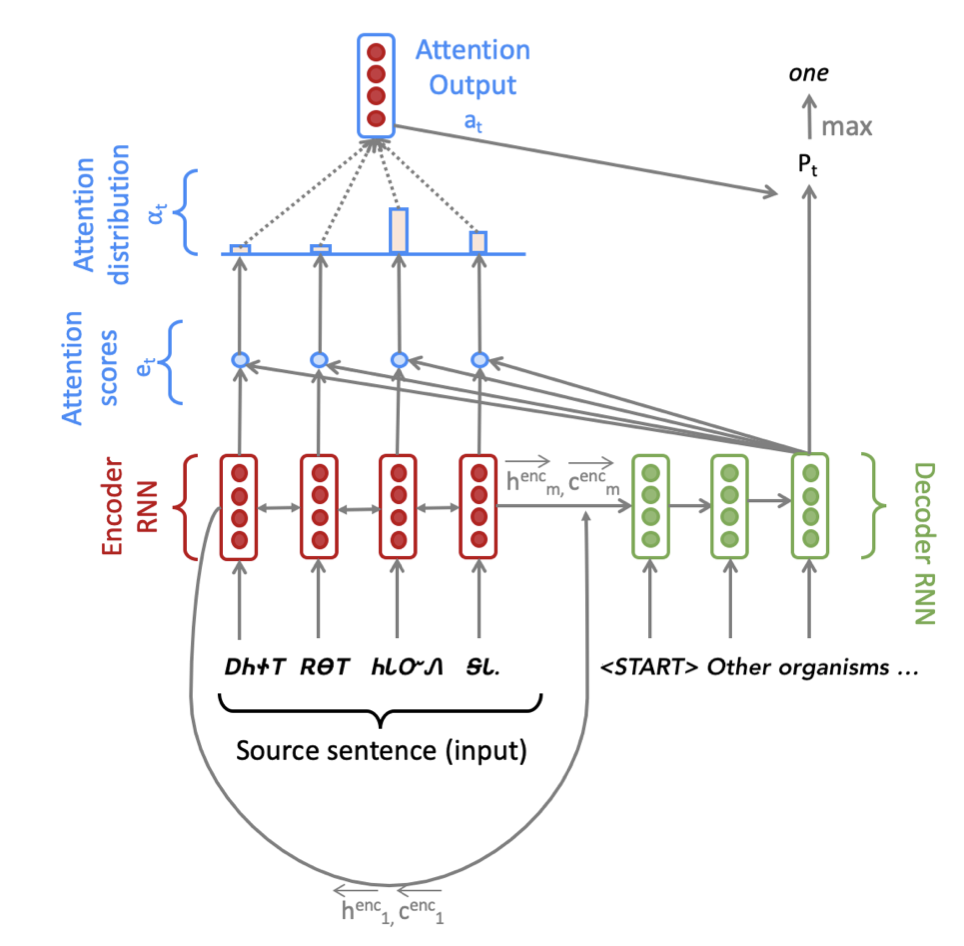
\includegraphics[width=0.7\textwidth]{images/nmt.png}
        \caption{Seq2Seq Model with Multiplicative Attention, shown on the third step of the decoder. Note that for readability, we do not picture the concatenation of the previous combined-output with the decoder input.}
        \label{nmt-figure}
    \end{center}
\end{figure}

\subsection*{Model description (training procedure)}
Given a sentence in the source language, we look up the word embeddings from an embeddings matrix, yielding $\bx_1, \dots, \bx_m \mid \bx_i \in \Real^{e \times 1}$, where $m$ is the length of the source sentence and $e$ is the embedding size. We feed these embeddings to the bidirectional Encoder, yielding hidden states and cell states for both the forwards ($\rightarrow$) and backwards ($\leftarrow$) LSTMs. The forwards and backwards versions are concatenated to give hidden states $\henc_i$ and cell states $\cenc_i$:
 
\begin{align}
    \henc_i = [\hencfw{i}; \hencbw{i}] \enspace &\text{where}\enspace \henc_i \in \Real^{2h \times 1}, \hencfw{i},\hencbw{i} \in \Real^{h \times 1} &1 \le i \le m \\
    \cenc_i = [\cencfw{i};\cencbw{i}] \enspace &\text{where} \enspace \cenc_i \in \Real^{2h \times 1}, \cencfw{i},\cencbw{i} \in \Real^{h \times 1} &1 \le i \le m
\end{align}

We then initialize the Decoder's first hidden state $\hdec_0$ and cell state $\cdec_0$ with a linear projection of the Encoder's final hidden state and final cell state.\footnote{If it's not obvious, think about why we regard $[\hencbw{1}, \hencfw{m}]$ as the `final hidden state' of the Encoder.}

\begin{align}
    \hdec_0 = \bW_{h}[\hencfw{m};\hencbw{1}] \enspace &\text{where} \enspace \hdec_0 \in \Real^{h \times 1}, \bW_{h} \in \Real^{h \times 2h}\\
    \cdec_0 = \bW_{c}[\cencfw{m};\cencbw{1}] \enspace &\text{where} \enspace \cdec_0 \in \Real^{h \times 1}, \bW_{c} \in \Real^{h \times 2h}
\end{align}

With the Decoder initialized, we must now feed it a matching sentence in the target language. On the $t^{th}$ step, we look up the embedding for the $t^{th}$ word,  $\by_t \in \Real^{e \times 1}$. We then concatenate $\by_t$ with the \textit{combined-output vector} $\bo_{t-1} \in \Real^{h \times 1}$ from the previous timestep (we will explain what this is later down this page!\@) to produce $\overline{\by_t} \in \Real^{(e+h) \times 1}$. Note that for the first target word (i.e. the start token) $\bo_{0}$ is a zero-vector. We then feed $\overline{\by_t}$ as input to the Decoder LSTM.

\begin{align}
    \hdec_t, \cdec_t = \text{Decoder}(\overline{\by_t}, \hdec_{t-1}, \cdec_{t-1}) \enspace &\text{where} \enspace \hdec_t \in \Real^{h \times 1}, \cdec_t \in \Real^{h \times 1}\\
\end{align}

We then use $\hdec_t$ to compute  multiplicative attention over $\henc_0, \dots, \henc_m$:

\begin{align}
    \be_{t, i} = (\hdec_t)^T\bW_{\text{attProj}}\henc_i \enspace &\text{where} \enspace \be_{t} \in \Real^{m \times 1}, \bW_{\text{attProj}}\in \Real^{h \times 2h} & 1 \le i \le m \\
    \alpha_t= \text{Softmax}(\be_t) \enspace &\text{where} \enspace \alpha_t \in \Real^{m \times 1}\\
    \ba_t = \sum_{i}^{m}\alpha_{t,i}\henc_i \enspace &\text{where} \enspace \ba_t \in \Real^{2h \times 1}
\end{align}    
 
We now concatenate the attention output $\ba_t$ with the decoder hidden state $\hdec_t$ and pass this through a linear layer, Tanh, and Dropout to attain the \textit{combined-output} vector $\bo_{t}$.

\begin{align}   
    \bu_{t} = [\hdec_t; \ba_{t}] \enspace &\text{where} \enspace \bu_t \in \Real^{3h \times 1} \\
    \bv_t = \bW_{u}\bu_t \enspace &\text{where} \enspace \bv_t \in \Real^{h \times 1}, \bW_{u} \in \Real^{h \times 3h}\\
    \bo_t = \text{Dropout}(\text{Tanh}(\bv_t)) \enspace &\text{where} \enspace \bo_t \in \Real^{h \times 1}
\end{align}

Then, we produce a probability distribution $\bP_t$ over target words at the $t^{th}$ timestep:

\begin{align}
    \bP_t = \text{Softmax}(\bW_{\text{vocab}}\bo_{t}) \enspace &\text{where} \enspace \bP_t \in \Real^{V_{t} \times 1}, \bW_{\text{vocab}} \in \Real^{V_{t} \times h}
\end{align}

Here, $V_{t}$ is the size of the target vocabulary. Finally, to train the network we then compute the softmax cross entropy loss between $\bP_t$ and $\bg_{t}$, where $\bg_{t}$ is the 1-hot vector of the target word at timestep $t$:

\begin{align}
    J_t(\theta) = CE(\bP_t,\bg_{t})
\end{align}

Here, $\theta$ represents all the parameters of the model and $J_t(\theta)$ is the loss on step $t$ of the decoder.
Now that we have described the model, let's try implementing it for Cherokee to English translation!

\subsection*{{\color{red} Setting up your Virtual Machine}}
Follow the instructions in the \href{https://docs.google.com/document/d/10J520Vnb1LnAMo0qgSYpG5cEEbomqQ371NIqg1IAv-4/edit?usp=sharing}{XCS224N Azure Guide} in order to create your VM instance. Though you will need the GPU to train your model, we strongly advise that you first develop the code locally and ensure that it runs, before attempting to train it on your VM. GPU time is expensive and limited. It takes approximately \textbf{30 minutes to 1 hour} to train the NMT system. We don't want you to accidentally use all your GPU time for the assignment, debugging your model rather than training and evaluating it. Finally, \textbf{make sure that your VM is turned off whenever you are not using it.}

In order to run the model code on your VM, please run the following command to create the proper virtual environment (You did this at the beginning of the course on your local computer):

\begin{lstlisting}
$ conda update -n base conda
$ conda env create --file environment.yml
\end{lstlisting}

If you have a local GPU, then instead of using |XCS224N| conda environment, create a new environment that supports GPU, |XCS224N_GPU| by following line:

\begin{lstlisting}
$ conda env create --file environment_gpu.yml
$ conda activate XCS224N_GPU
\end{lstlisting}

For local development and testing, you can feel free to continue to using the same |XCS224N| environment you've used for all the assignments so far.

\subsection*{Implementation Assignment}

\begin{enumerate}[(a)]
    \item \points{1a} In order to apply tensor operations, we must ensure that the sentences in a given batch are of the same length. Thus, we must identify the longest sentence in a batch and pad others to be the same length. Implement the \texttt{pad\_sents} function in \texttt{submission/utils.py}, which shall produce these padded sentences.

    \item \points{1b} Implement the \texttt{\_\_init\_\_} function in \texttt{submission/model\_embeddings.py} to initialize the necessary source and target embeddings.

    \item \points{1c} Implement the \texttt{\_\_init\_\_} function in \texttt{submission/nmt\_model.py} to initialize the necessary layers (LSTM, projection, and dropout) for the NMT system.

    \item \points{1d} Implement the \texttt{encode} function in \texttt{submission/nmt\_model.py}. This function converts the padded source sentences into the tensor $\bX$, generates $\henc_1, \dots, \henc_m$, and computes the initial state $\hdec_0$ and initial cell $\cdec_0$ for the Decoder.

    \item \points{1e} Implement the \texttt{decode} function in \texttt{submission/nmt\_model.py}. This function constructs $\bar{\by}$ and runs the \texttt{step} function over every timestep for the input.

    \item \points{1f} Implement the \texttt{step} function in \texttt{submission/nmt\_model.py}. This function applies the Decoder's LSTM cell for a single timestep, computing the encoding of the target word $\hdec_t$, the attention scores $\be_t$, attention distribution $\alpha_t$, the attention output $\ba_{t}$, and finally the combined output $\bo_t$.

    Now it's time to get things running! Execute the following to generate the necessary vocab file (you can do this on your local computer):
\begin{lstlisting}
(XCS224N)$ sh run.sh vocab
\end{lstlisting}
    As noted earlier, we recommend that you develop the code on your personal computer.  Confirm that you are running in the proper conda environment and then execute the following command to train the model on your local machine:
\begin{lstlisting}
(XCS224N)$ sh run.sh train_local
\end{lstlisting}
    Once you have ensured that your code does not crash (i.e. let it run until \texttt{iter 10} or \texttt{iter 20}), power on your VM from the Azure Web Portal. Then read the \textit{Practical Guide for Using the VM} section of the \href{https://docs.google.com/document/d/10J520Vnb1LnAMo0qgSYpG5cEEbomqQ371NIqg1IAv-4/edit?usp=sharing}{XCS224N Azure Guide} for instructions on how to upload your code to the VM.
    Next, turn to the \textit{Managing Processes on a VM} section of the Practical Guide and follow the instructions to create a new tmux session. Concretely, run the following command to create tmux session called \texttt{nmt}.
\begin{lstlisting}
(XCS224N_GPU)$ tmux new -s nmt
\end{lstlisting}
    Once your VM is configured and you are in a tmux session, reactivate your |XCS224N| environment and execute. Note that it is a different conda env |XCS224N_GPU| based on |environment_gpu.yml|. Details can be found from \href{https://docs.google.com/document/d/10J520Vnb1LnAMo0qgSYpG5cEEbomqQ371NIqg1IAv-4/edit?usp=sharing}{XCS224N Azure Guide}.
\begin{lstlisting}
$ conda activate XCS224N_GPU
(XCS224N_GPU)$ sh run.sh train
\end{lstlisting}
    Once you know your code is running properly, you can detach from session and close your ssh connection to the server. To detach from the session, run:
\begin{lstlisting}
(XCS224N_GPU)$ tmux detach
\end{lstlisting}
    You can return to your training model by ssh-ing back into the server and attaching to the tmux session by running:
\begin{lstlisting}
(XCS224N_GPU)$ tmux a -t nmt
\end{lstlisting}
    \item \points{1g} Once your model is done training (\textbf{this should take about 30 minutes to 1 hour on the VM}), execute the following command to test the model:
\begin{lstlisting}
(XCS224N_GPU)$ sh run.sh test
\end{lstlisting}

    After running this command, it should generate a file |src/submission/test_outputs.txt| needed for submission.

\end{enumerate}
\clearpage

\textbf{Deliverables}

For this assignment, please submit all files within the |src/submission| subdirectory.  This includes:
\begin{itemize}
    \item |src/submission/__init__.py|
    \item |src/submission/model_embeddings.py|
    \item |src/submission/nmt_model.py|
    \item |src/submission/utils.py|
    \item |src/submission/test_outputs.txt|
\end{itemize}   
